\begin{problem}[问题5.1]一虹吸管放于水桶中, 其位置如
\vspace{-2em}
\begin{multicols}{2}
~

右图所示. 如果水桶及虹吸管的截面积分别为$A$和$B$, 且$A\gg B$, 试计算虹吸管的流量. 水看作是理想不可压缩的, 且受重力作用, 运动是定常的.
\begin{center}
\usetikzlibrary{%
    decorations.pathreplacing,%
    decorations.pathmorphing,arrows
}
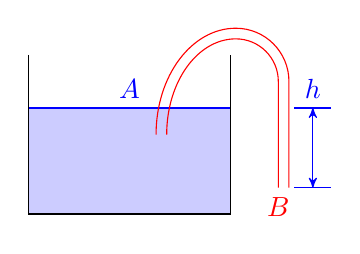
\begin{tikzpicture}[scale=1.35]
\fill[blue!20](-0.25,1)--(-0.25,0)--(1.65,0)--(1.65,1);
\draw[blue](-0.25,1)--(1.65,1) node[midway,above]{$A$};
\draw[semithick](-0.25,1.5)--(-0.25,0)--(1.65,0)--(1.65,1.5);

\draw[red](0.95,0.75) arc(180:90:0.75 and 1) arc(90:0:0.5) --(2.2,0.25) ;

\draw[red](1.05,0.75) arc(180:90:0.65 and 0.9) arc(90:0:0.4) --(2.1,0.25)node[below]{$B$};

\draw[blue](2.25,1)--(2.6,1) (2.25,0.25)--(2.6,0.25);

\draw[blue,<->,>=stealth'] (2.425,0.25)--(2.425,1) node[above]{$h$}; 

\end{tikzpicture}

%\includegraphics[width=0.28\textwidth]{./figures/problem01.pdf}
\end{center}
\end{multicols}
\end{problem}

\begin{solution}
\textbf{解:}对$A$, $B$面应用Bernoulli方程
\[
\frac{1}{2}v_A^2 + \frac{p_A}{\rho} + gz_A =
\frac{1}{2}v_B^2 + \frac{p_B}{\rho} + gz_B
\]
由质量守恒$Av_A = Bv_B$及$A\gg B$, 可知$v_A\rightarrow 0$. 又知$p_A = p_B = p_0$及$z_A-z_B = h$. 因此上式可化为
\[
\frac{1}{2}v_B^2 = g(z_A-z_B) = gh \Longrightarrow  v_B = \sqrt{2gh}
\]
因此,$A$,$B$两液面高度差为$h$时流量为
\[
q = Bv_B = B\sqrt{2gh}
\]
若考虑到随着水流从$B$口不断流出, $A$, $B$液面差$H(t)$(为也$h$区分,这里使用$H(t)$, $H(0) = h$)将非常缓慢的变小, $v_B(t)$也缓慢变化. 有如下关系
\[
Av_A = Bv_B\Longrightarrow -A\frac{d(H)}{dt} = Bv_B(t) \Longrightarrow A\frac{dH}{dt} = -B\sqrt{2gH}
\Longrightarrow \frac{dH}{\sqrt{H}} = -\frac{B}{A}\sqrt{2g}dt
\]
考虑到$h(0)=h$积分得
\[
H(t) = \Big[\sqrt{h}-\frac{B}{2A}\sqrt{2g}t\Big]^2
\]
因此, 流量是时间的函数
\[
q(t) = B\sqrt{2gH(t)} = B\Big(\sqrt{2gh}-\frac{B}{A}gt\Big)
\]

\end{solution} 
